%%%%%%%%%%%%%%%%%%%%%%%%%%%%%%%%%%%%%%%% Klasse Festlegen
%\documentclass[Master,BMR,english]{BASE/twbook}
\documentclass[Bachelor, BIC, english, fhCitStyle, IEEE]{BASE/twbook} % FH definierte Zitierstandards verwenden
%%%%%%%%%%%%%%%%%%%%%%%%%%%%%%%%%%%%%%%% Verwendete Packages
\usepackage[utf8]{inputenc} % Zeichen-Enkodierung (evtl. Abweichungen für Apple)
\usepackage[T1]{fontenc} % Zeichen-Enkodierung
\usepackage{blindtext} % Platzhaltertexte
\usepackage{minted} % Darstellung von Code
\usepackage{comment} % Auskommentieren von ganzen Passagen
\usepackage{csquotes}
\usepackage{algorithm} % Umgebung f Algorithmen
\usepackage[noend]{algpseudocode}
\graphicspath{ {./PICs/} }
% Wenn Sie während Ihrer Arbeit
% merken, dass Sie zusätzliche Funktionen
% benötigen ist hier ein guter Platz um
% weitere Packages zu laden
%%%%%%%%%%%%%%%%%%%%%%%%%%%%%%%%%%%%%%%% Zitierstil zum selbst definieren
\usepackage[backend=biber, style=ieee]{biblatex} % LaTeX definierter IEEE- Standard
%\usepackage[backend=biber, style=authoryear]{biblatex}      % LaTeX definierter Harvard-Standard
\addbibresource{Literature.bib} % Literatur-File definieren
%%%%%%%%%%%%%%%%%%%%%%%%%%%%%%%%%%%%%%%% Custom commands
% Redefine \section, \subsection, \subsubsection to not add entries to the ToC
% Define a command to temporarily disable \addcontentsline
\newcommand{\nocontentsline}[3]{}
% Define commands to create sections, subsections, and subsubsections without ToC entries
\newcommand{\hidsection}[1]{\bgroup\let\addcontentsline=\nocontentsline\section{#1}\egroup}
\newcommand{\hidsubsection}[1]{\bgroup\let\addcontentsline=\nocontentsline\subsection{#1}\egroup}
\newcommand{\hidsubsubsection}[1]{\bgroup\let\addcontentsline=\nocontentsline\subsubsection{#1}\egroup}
% Defines an alias for writing inline monospace font for code related things
\def\code#1{\texttt{#1}}
%%%%%%%%%%%%%%%%%%%%%%%%%%%%%%%%%%%%%%%% Einträge für Deckblatt
\title{Precision at Pixel-Level:\\\acl{yoloAlt} doing UI test automation}

\author{Nikolaus Rieder}
\studentnumber{2010258028}
%\author{Titel Vorname Name, Titel\and{}Titel Vorname Name, Titel}
%\studentnumber{XXXXXXXXXXXXXXX\and{}XXXXXXXXXXXXXXX}

\supervisor{Dr. Dietmar Millinger}
%\supervisor[Begutachter]{Titel Vorname Name, Titel}
%\supervisor[Begutachterin]{Titel Vorname Name, Titel}
%\secondsupervisor{Titel Vorname Name, Titel}
%\secondsupervisor[Begutachter]{Titel Vorname Name, Titel}
%\secondsupervisor[Begutachterinnen]{Titel Vorname Name, Titel}

\place{Wien}
%%%%%%%%%%%%%%%%%%%%%%%%%%%%%%%%%%%%%%%% Danksagung/Kurzfassung/Schlagworte
% Abstract
\outline{ Developing and executing test suites on embedded devices with a \ac{gui} can be a time-consuming and exhaustive process. Nevertheless, it is a necessary task in interfaces of critical infrastructure, like \ac{fas} or \ac{hcs} developed at Schrack Seconet. This research analyzes the viability of using machine learning for identifying and detecting \ac{ui} widgets based purely on screenshot data. The analysis is written from the perspective of \ac{ta} performed on critical systems like the aforementioned. The focus is on high performing results due to the qualitative requirements in \ac{ui} test automation of such systems, where upcoming problems during development are considered potentially critical if not detected. \\ During paper development, a \ac{yolo} model was trained on randomly synthesized datasets of \ac{ui} screenshots. The datasets were generated with the \ac{lvgl}, a common and popular library in embedded systems. During development of the datasets and model training processes, key problem factors are identified and potential mitigations addressed. The findings showcase these points in the context of a nurse call system, where reliability of the user interface plays a critical role and margin for error is non-existent. \\ The project follows a Design Science research approach, in which a \ac{ui} generator for \ac{lvgl} was created, that is capable of generating datasets of randomly chosen and placed widgets on a screen, as well as the generation of realistic looking designs by using a system based on a \ac{json} schema. In order to create larger datasets, a \ac{llm} was used to design multiple \ac{ui}s from a list of pre-defined contexts and themes. \\\\ This research aims to reduce time spent in test development and improve test coverage of varied \ac{ui}s in devices of critical systems, while aiding human developers in manual and automated testing. \\ }
\keywords{YOLOv8, UI Testing, embedded devices, widget detection, widget
classification, automated testing}
% Acknowledgements
\acknowledgements{I extend my gratitude to the faculty and staff at UAS Technikum Vienna for their invaluable guidance and the wealth of knowledge they have shared, which has culminated in the completion of this bachelor thesis. Special appreciation is given to my academic advisor, Dietmar Millinger, for his expertise and dedication. Additional thanks are due to Dietmar Millinger, Karl M. Göschka, Lorenz Froihofer, and Susanne Teschl for their inspiration and exceptional contributions to my understanding of machine learning, computer science, and mathematics, respectively. Thanks should also go to my academic peers, for the collaborative environment fostered on our student community server and the valuable networks we have built throughout this educational journey. I am particularly grateful to my partner, whose support and patience were unwavering during my academic endeavors at the UAS Technikum Vienna. I would also like to express my sincere thanks to Schrack Seconet AG for providing me with the opportunity to develop this paper in a professional context. The support from colleagues has been instrumental in aligning my academic pursuits with practical applications in the workplace. Lastly, I thank my own body and mind for not breaking apart throughout the long days and mostly nights that were involved up to this point.}
\setListingsAndAcronyms % Definition der Namen für Quellcodeverzeichnis
%%%%%%%%%%%%%%%%%%%%%%%%%%%%%%%%%%%%%%%%%%%%%%%%%%%%%%%%%%%%%% End of header
%%%%%%%%%%%%%%%%%%%%%%%%%%%%%%%%%%%%%%%%%%%%%%%%%%%%%%%%%%%%%% Start of document
\begin{document}
%%%%%%%%%%%%%%%%%%%%%%%%%%%%%%%%%%%%%%%% Title page in FHTW style
\maketitle
%%%%%%%%%%%%%%%%%%%%%%%%%%%%%%%%%%%%%%%%%%%%%%%%%%%%%%%%%%%%%% Start of content
%%%%%%%%%%%%%%%%%%%%%%%%%%%%%%%%%%%%%%%% Start of Introduction
\chapter{Introduction}
In embedded systems providing critical infrastructure, it is often mandatory to have well-established and good testing procedures. One such system is nurse call used in hospitals and health care facilities, which consists of devices that allow humans to call for help in situations ranging from mundane \textit{(e.g. requesting patient service)} to life-threatening \textit{(e.g. cardiac arrest alarm)} use-cases. These systems require interfaces for human interaction and such interfaces need to be rigorously tested, to provide feedback on system quality in early stages of development, where the potential for harm is very low. Additionally, automated testing becomes necessary, to reduce possible variation in test execution when compared to manual testing, where human-error is more prevalent than with machines repeating test cases.\\
However, when such interfaces only consist of a touch display, it can become very challenging to automate, as it requires tools for the machine to analyze the visual image and to interact with the \ac{ui} using stimuli \textit{(e.g. simulated touch)}. The automation gets further complicated, the more inputs and outputs the machine needs to deal with in order to perform a representative human test routine. Once such test routines are established, they need to be continously maintained in order to adapt to changes to the \ac{ui}, otherwise such changes can break the test system and halt the overall development process.\\
This research project will demonstrate a machine learning tool to aid in analyzing images to obtain metadata about the displayed \ac{ui}. The metadata consists of position and size of individual widgets, which then can be used in testing routines for precise functional interactions. By training a model that can detect and classify widgets based on screenshots, the testing routines can adapt to many \ac{ui} arrangements dynamically, which can reduce labor involved for maintenance of test repositories.\\
Since covering all possible \ac{ui} libraries and frameworks would be tremendous in scope, the research will limit focus on \ac{lvgl} as the basis for the \ac{ui}. It begins by creating an image and annotation generator for \ac{lvgl}, since there is no available dataset for this library specifically and it also allows for targeted adjustments in dataset size, variation and balance of widget types. Furthermore, it allows for validation based on a real world example from the company where the author is employed at. The work will also be limited to a subset of available widget types, to provide a basic baseline for the viability of the tool, which may be easily extended in the future.\\
Once dataset creation is automated, the paper will demonstrate training based on the \ac{yolo} model and evaluate performance in comparison to human methods. From a testing perspective, this paper is most concerned with the prediction accuracy of the model, since a tool that is not capable of reliable detection will only shift maintenance problems to the tool itself, rather than improving them overall.
%%%%%%%%%%%%%%%%%%%%%%%%%%%%%%%%%%%%%%%%%%%%%%%%%%%%%%%%%%%%%%%%%%
\clearpage
%%%%%%%%%%%%%%%%%%%%%%%%%%%%%%%%%%%%%%%% Start of Problem description
\chapter{Problem description}
When developing automated test cases for a product which has very long life cycles, due to being incorporated in building infrastructure, of 10 years or more, it can be expected that involved maintenance labor of existing test cases surpasses the creation of new test cases. But even in such long-lasting products, big system changes \textit{(e.g. \ac{ui} redesign, new controller architecture, ...)} eventually occur. Such a change incurs a new evaluation and design of existing test procedures, to accommodate for the new system or \ac{ui}, even if the actual use-case and performed steps fundamentally remain the same.
For the business it is therefor beneficial to have testing tools, which reduce the maintenance costs of such legacy test costs, by being dynamic and adaptable to the given test environment.\\
% THIS PART requires more research in the literature to write a more coherent problem description
% I DON'T EVEN KNOW IF I NEED THIS PART
% Such a change incurs a new evaluation and design of existing test procedures, to accommodate for the new system or \ac{ui}, even if the actual use-case and performed steps fundamentally remain the same. The development of a breaking change must then factor in the costs of changing legacy tests and it may result in decisions that will have less test quality as a result, in favor of bringing in more money for the business.\\
% Therefor it can be beneficial for the tester to make use of tools, which reduce development costs incurred.
% When developing test cases for \aclp{ui}, it is necessary to differentiate between white-box and black-box testing. A white-box testing approach would incorporate knowledge about the code of the \ac{ui}, where a tester would know about the types of widgets used and their applied properties, amongst other things related to the contents of the source. This testing approach is typically used in unit and early integration testing, possibly performed by the developer themselves. In black-box testing, such information is completely stripped away and it is best-practice to leave such work to people outside of the development team to avoid confirmation-bias. % TODO citations for testing approaches, best-practice, etc.
% The context of this paper focuses on the latter with the limitation, that the author has knowledge of the library used and the hardware product itself. The author is a professional in testing and test automation, aware of the risks involved when it comes to knowledge about inner workings of the system under test. % TODO citation of involved risks due to confirmation bias
% As such, the main input for the tool will be limited to what is accessible to the tester, which is constrained to be a black-box testing approach.\\
\section{Problem context at Schrack Seconet}
\clearpage
%%%%%%%%%%%%%%%%%%%%%%%%%%%%%%%%%%%%%%%% Start of research questions
\chapter{Research questions}
% need to properly define this part
\clearpage
%%%%%%%%%%%%%%%%%%%%%%%%%%%%%%%%%%%%%%%% Start of literature & theory
\chapter{Existing literature and theoretical basis}
\hidsection{\acf{cnn}}
\hidsubsection{\acf{yolo} architecture}
\hidsection{\acf{lvgl}}
\clearpage
%%%%%%%%%%%%%%%%%%%%%%%%%%%%%%%%%%%%%%%% Start of generator development
\chapter{Development of synthesized datasets}
There generally is no available dataset for the target graphics library (\ac{lvgl}) of this research, so it was mandatory to create one during project development. Creating such a dataset artificially, meaning the images are not based on real world \acp{ui}, has the benefit of being able to adjust the size, variation and balance of the dataset very precisely. It would however be a complicated and time-consuming endeavour, if all of these \aclp{ui} would be created manually using regular \ac{lvgl} code, given that typical datasets for a \ac{ml} model of this type require hundreds of pictures or even more.\\
This is why a generator must be built, which is capable of creating and placing widgets in a structured manner. A screenshot of the displayed window needs to be captured and any metadata (size and position) of placed widgets must be gathered for creating corresponding annotations. The generator will also need to handle variation in visual representation of widgets, otherwise resulting datasets would be biased and detection accuracy of the model would be bad when used on screenshots of real-world examples, which typically incorporate varying visual representations of the same widget type.\\
In order to create variety in individual widgets, a randomized approach is used, where the outputted widgets will have varying styles applied to them. To gain more fine-control on the final visual representation of an created \ac{ui}, an additional design mode is necessary, where the creation of user interfaces can be statically described. The design mode will allow for creation of realistically looking \acp{ui}, while the random mode will allow for the creation of varying visual representation of the individual widgets.\\
Since the creation of a window with corresponding in \ac{lvgl} is typically singular, it will be necessary to have a mechanism to repeatedly call the generator to obtain a new image with each iteration. Using a modular approach, this paper will separate the generator, capable of producing a single image with annotations, from the the so-called randomizer, which will loop the generator repeatedly for an arbitrary amount of iterations. This approach allows for a focused implementation that is capable of producing a good singular image, while having a secondary implementation that solely focuses on the organisation and creation of the dataset. Additionally, when written in the modular approach, it also allows for separation of concerns, where the generator will only need to deal with the intricacies of the \ac{lvgl} API, while the randomizer can focus on the structural requirements of the dataset for the chosen model.\\
\section{First generator version in C}
The initial generator (v1) is forked from the existing VSCode simulator project of \ac{lvgl}. The simulator was stripped from any demo code and re-used as a binary with \ac{cli} arguments. For proper operation, the \code{lv\_conf.h} file was also modified, to increase allocation memory and deactivate unnecessary features. In the configuration, the default color depth was also modified to be 24 bit, so that output images would appear in higher quality. To be able to store screenshots, an additional library named \code{lv\_100ask\_screenshot} was used, which deals with the proper JPEG encoding using the \code{tiny\_jpeg} library.\\
Since the generator uses the allocation and storage mechanisms provided by \ac{lvgl}, it is necessary to use an identifier for the target storage system as prefix to the output filename. For this the \code{\textbackslash} character was chosen, so when supplying the \ac{cli} with a desired output filename, an example argument would look like this: \code{\textbackslash screenshot.jpg}\\
The following usage information will explain the available console arguments for this generator version:
\begin{listing}[htbp]
    \begin{minted}[
        frame=single,
        framesep=2mm,
        baselinestretch=1.2,
        bgcolor=white,
        fontsize=\footnotesize,
        breaklines
        ]{shell-session}
Usage: ./lvgl_ui_generator/build/bin/demo [OPTIONS]
Options:
-m <mode>                   Set the operation mode ("randomizer" or "design")
Randomizer Mode Options:
-w <width>                  Set the width of the UI
-h <height>                 Set the height of the UI
-c <widget_count>           Set the number of widgets to be randomized
-t <widget_types>           Comma-separated list of widget types to be used
-o <output_file>            Set the output file path
-d <delay_count>            Set the screenshot delay count
-l <layout>                 Set the layout type
    \end{minted}
    \caption{Usage instructions of LVGL generator v1}
\end{listing}
\\
\begin{figure}
    \caption{Example output of generator v1 (640x640, 40 random widgets)}
    \centering
    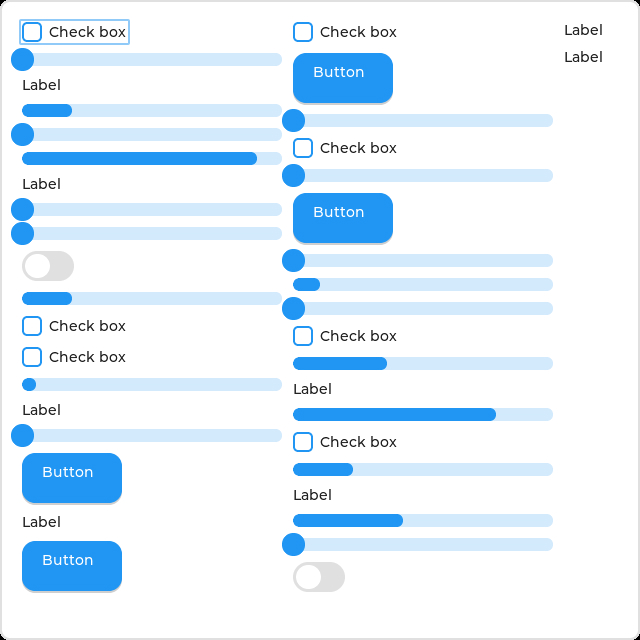
\includegraphics[width=\textwidth]{generator_v1_example.jpg}
    \label{fig:genv1example}
\end{figure}
When run, the generator will produce an image in the provided width and height. Fig. \ref{fig:genv1example}\\It will place randomly chosen widgets up to the given count on the window and use the selected layout (none, grid, flex) to structure them.
\\
The layout structuring of widgets helped in outputting more placement variation in the final image. When using \code{flex}, the created widgets are aligned and will wrap onto the next line if they run out of width. In the \code{grid} layout, widgets would be placed in a grid-like pattern over the whole image. Finally in the \code{none} layout, widgets would be absolutely positioned randomly over the screen, sometimes also causing overlap of widget types.
\clearpage
\subsection{Development issues}
During development and testing of the first generator, it became apparent, that implementing further widget types would create a lot of complexity due to parameter passing in code. Since the C language does not inherently have classes, it was considered to be much more difficult to implement multiple widget types, each of which require a different set of options to be displayed properly.\\
Additionally, issues like segmentation faults due to window deletion occurred, which were inherited from the forked project. The implementation of a design mode was attempted, but this only increased complexity, which resulted in more unreliability of the program, despite the authors experience in the language. Frequent errors in compilation as well as a high compilation time due to the included \ac{lvgl} examples, which the author was not able to remove, were halting and slowing down development time. A lot of features \textit{(widget styles and states, widget property randomization, ...)} were still left to be implemented at a low level and C being a systems programming language, it was becoming too big of a problem for the project.\\\\
The general implementation based on C proved to be much more error-prone as a result of these issues and was therefor considered too complex for usage in a generation pipeline. A new solution was sought after, which would allow implementation of the generator in a more resilient and forgiving programming language.\\
\ac{lvgl} provides C bindings for usage and implementation in other programming languages. A language promoted by the creators themselves is micropython, which is a reduced implementation of python for running on hardware. While the issues faced with the initial generator certainly are solvable, there existed no premise to continue in the C language. A new version in that language was considered to be a simpler approach that would refocus the project on the dataset creation matter at hand.
\clearpage
\section{Second generator version in Micropython}
The second generator version is implemented in micropython, and was started as a fresh project using the \code{lv\_micropython} project as a necessary sub-module for compiling the micropython binary including the \code{lv\_bindings} module.\\
Rewriting the functionality of the initial generator was much simpler, as the binary comes with \code{argparse} for easily creating a \ac{cli} interface. Having the functionality of classes, it was also easier to differentiate between the two modes with their own source files. Widget creation was divided into separate functions, one for each widget type, and then called via a mapping of the type name to the creation function. This proved to be much more maintainable throughout project development and issues were able to be faced on an individual basis per implemented type.\\
Both modes provide a function to retrieve the top-level container and all its children in a dictionary object format, containing all relevant metadata information gathered through usage of the \code{coords\_t} object. This \ac{lvgl} object is necessary, as it stores the coordinates of a widget in relation to the whole window, while other methods usually provide this information in relation to the parent container that the widget resides in.\\
The retrieved container is passed to a screenshot function, which uses a manually added JPEG encoding from the tinyjpeg project to create an image. Using the coordinate metadata, the annotation file of the resulting image is created in \ac{yolo} format (\code{class center\_x center\_y center\_width center\_height}) and also normalized if the user provides the corresponding flag.
A resulting example image using design mode is illustrated in Fig.\ref{fig:genv2example} and its corresponding annotation file is listed below.
\begin{figure}
    \caption{Example output of generator v2 (640x640, widget\_showcase.json)}
    \centering
    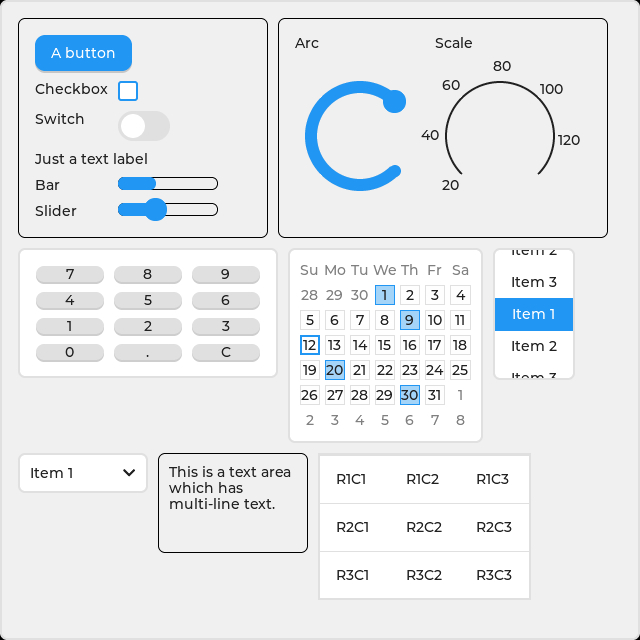
\includegraphics[width=\textwidth]{generator_v2_example.jpg}
    \label{fig:genv2example}
\end{figure}
\begin{listing}[htbp]
    \begin{minted}[
        frame=single,
        framesep=2mm,
        baselinestretch=1.2,
        bgcolor=white,
        fontsize=\footnotesize
        ]{shell-session}
textarea 0.3625 0.784375 0.234375 0.15625
table 0.6625 0.821875 0.3328125 0.2296875
checkbox 0.2046875 0.140625 0.04375 0.03125
arc 0.5609375 0.2109375 0.203125 0.203125
label 0.0734375 0.2875 0.0390625 0.025
label 0.0859375 0.328125 0.065625 0.025
label 0.478125 0.065625 0.0375 0.025
label 0.7078125 0.065625 0.059375 0.025
label 0.1109375 0.1375 0.1140625 0.025
bar 0.2609375 0.2859375 0.15625 0.0203125
label 0.0921875 0.184375 0.078125 0.025
label 0.1421875 0.246875 0.1765625 0.025
switch 0.2234375 0.1953125 0.08125 0.046875
buttonmatrix 0.2296875 0.4875 0.40625 0.203125
button 0.1296875 0.08125 0.1515625 0.05625
calendar 0.6015625 0.5390625 0.3046875 0.3046875
scale 0.7796875 0.2109375 0.203125 0.203125
slider 0.2609375 0.3265625 0.15625 0.0203125
roller 0.8328125 0.4890625 0.128125 0.20625
dropdown 0.128125 0.7375 0.203125 0.0625
    \end{minted}
    \caption{Usage instructions of LVGL generator v1}
\end{listing}
\clearpage
\hidsubsection{Distorted output images due to render race conditions}
The used snapshot API sometimes causes output issues, since race-conditions can occur due to render updates while the referenced image data is still being encoded, resulting in distorted or sheared images. This largely originates from adding the JPEG encoding in micropython, which inherently is much slower than its C counterpart. While the issue was not solved during paper development due to its late discovery, a problem solution using a compiled C module of the latest tinyjpeg version was discussed in development forums of \ac{lvgl}. Adding this module will improve encoding speed and thus not face race conditions due to underlying render updates by \ac{lvgl}. Images which had this issue needed to be regenerated and datasets were fixed manually.
\hidsubsection{Memory allocation errors}
Since the image encoding takes place in micropython, it actually takes up a lot more memory in heap. When creating and encoding images with the generator, it may result in memory allocation errors, depending on available memory on the running machine. This issue is not solved in the final generator version of the paper and was circumvented by retry mechanisms when creating image files using the dataset pipeline.
\section{Random mode}
In random mode, the generator will produce a window of desired width and height. It randomly chooses widgets from the user provided type list and places them into a container. Since absolute positioning proved to be most suitable for random generation, the implementation of layouts was omitted. To avoid overlap, a spatial map was used, to find free space in the window during widget creation and placement.\\
The usage description in Listing \ref{code:genv2usage} provides an overview of the parameters for this mode.
\begin{listing}[htbp]
    \begin{minted}[
        frame=single,
        framesep=2mm,
        baselinestretch=1.2,
        bgcolor=white,
        fontsize=\footnotesize,
        breaklines
        ]{shell-session}
usage: src/main.py [-h] [-m, --mode mode] [-?, --usage] [-n, --normalize] [-o, --output_file output_file] [-W, --width width] [-H, --height height] [-c, --widget_count widget_count] [-t, --widget_types widget_types+] [-l, --layout layout] [--random-state]

Process CLI arguments for the UI generator.

optional args:
  -h, --help                        show this message and exit
  -m, --mode                        mode the mode to run the program in
  -?, --usage                       Print usage information for that mode.
  -n, --normalize                   normalize the bounding boxes
  -o, --output_file output_file     The output file (screenshot)
  -W, --width width                 the width of the UI
  -H, --height height               the height of the UI
  -c, --widget_count widget_count   the count of widgets
  -t, --widget_types widget_types+  A list of widget types
  -l, --layout layout               the layout option
  --random-state                    Use a random state for each created widget (experimental)
    \end{minted}
    \caption{Usage instructions of LVGL generator v2 in random mode}
    \label{code:genv2usage}
\end{listing}\\\\
\subsection{Style and state variation}
When using random mode, the generator will randomize applied style of widgets to artificially create variation in created datasets. Additionally, there is an experimental feature, which will also randomize the state of widgets. The latter is not recommended for usage in training, as sometimes this might cause widgets to not be displayed if their state is invalid or disabled, which will confuse the model, as the created metadata will still include the annotation of said widget.\\
Listing \ref{code:randomized-properties} shows the properties and their range of possible values to be randomized. Listing \ref{code:randomized-state} shows the available states.
\begin{listing}[htbp]
    \begin{minted}[
        frame=single,
        framesep=2mm,
        baselinestretch=1.2,
        bgcolor=white,
        fontsize=\footnotesize,
        breaklines
        ]{python}
# List of style properties to randomize
properties = [
    ('set_bg_color', lv.color_make),
    ('set_bg_opa', lambda: random.randint(0, 100)),
    ('set_border_color', lv.color_make),
    ('set_border_opa', lambda: random.randint(0, 100)),
    ('set_border_width', lambda: random.randint(0, 10)),
    ('set_outline_width', lambda: random.randint(0, 10)),
    ('set_outline_color', lv.color_make),
    ('set_outline_opa', lambda: random.randint(0, 100)),
    ('set_shadow_width', lambda: random.randint(0, 15)),
    ('set_shadow_offset_x', lambda: random.randint(0, 10)),
    ('set_shadow_offset_y', lambda: random.randint(0, 10)),
    ('set_shadow_color', lv.color_make),
    ('set_shadow_opa', lambda: random.randint(0, 100)),
    ('set_line_width', lambda: random.randint(0, 10)),
    ('set_line_dash_width', lambda: random.randint(0, 10)),
    ('set_line_dash_gap', lambda: random.randint(0, 10)),
    ('set_line_rounded', lambda: random.choice([True, False])),
    ('set_line_color', lv.color_make),
    ('set_line_opa', lambda: random.randint(0, 100)),
    ('set_text_color', lv.color_make),
    ('set_text_opa', lambda: random.randint(0, 100)),
    ('set_text_letter_space', lambda: random.randint(0, 10)),
    ('set_text_line_space', lambda: random.randint(0, 10)),
    ('set_opa', lambda: random.randint(0, 100)),
    ('set_align', lambda: random.choice([lv.ALIGN.CENTER, lv.ALIGN.TOP_LEFT, lv.ALIGN.TOP_RIGHT, lv.ALIGN.TOP_MID, lv.ALIGN.BOTTOM_LEFT, lv.ALIGN.BOTTOM_RIGHT, lv.ALIGN.BOTTOM_MID, lv.ALIGN.LEFT_MID, lv.ALIGN.RIGHT_MID, lv.ALIGN.DEFAULT])),
    ('set_pad_all', lambda: random.randint(0, 10)),
    ('set_pad_hor', lambda: random.randint(0, 10)),
    ('set_pad_ver', lambda: random.randint(0, 10)),
    ('set_pad_gap', lambda: random.randint(0, 10)),
    ('set_pad_top', lambda: random.randint(0, 10)),
    ('set_pad_bottom', lambda: random.randint(0, 10)),
    ('set_pad_left', lambda: random.randint(0, 10)),
    ('set_pad_right', lambda: random.randint(0, 10)),
    ('set_pad_row', lambda: random.randint(0, 10)),
    ('set_pad_column', lambda: random.randint(0, 10)),
    ('set_margin_top', lambda: random.randint(0, 10)),
    ('set_margin_bottom', lambda: random.randint(0, 10)),
    ('set_margin_left', lambda: random.randint(0, 10)),
    ('set_margin_right', lambda: random.randint(0, 10))
]
    \end{minted}
    \caption{Available style properties which are randomized in given value range}
    \label{code:randomized-properties}
\end{listing}
\begin{listing}[htbp]
    \begin{minted}[
        frame=single,
        framesep=2mm,
        baselinestretch=1.2,
        bgcolor=white,
        fontsize=\footnotesize,
        breaklines
        ]{python}
def randomize_state(widget: lv.obj):
    if hasattr(widget, "set_state"):
        state = random.choice([lv.STATE.CHECKED, lv.STATE.DISABLED, lv.STATE.FOCUSED, lv.STATE.PRESSED, lv.STATE.HOVERED, lv.STATE.EDITED])
        widget.set_state(state, True) # Add the state
    else:
        raise AttributeError(f"Widget {widget} does not have a 'state' property.")
    \end{minted}
    \caption{Available state properties which are randomized in given options}
    \label{code:randomized-state}
\end{listing}
\clearpage
\section{Design mode}
\subsection{Design contexts and themes}
\subsection{JSON schema}
\section{Dataset creation}
\subsection{Third-party integrations} % ClearML & LLM (ChatGPT)
\hidsubsubsection{Integration with ClearML}
\hidsubsubsection{Integration with LLM (gpt-4-turbo)}
\clearpage
%%%%%%%%%%%%%%%%%%%%%%%%%%%%%%%%%%%%%%%% Start of model training
\chapter{Training of YOLO model}
\section{Training pipeline}
\subsection{Training agent on Google Colab}
\section{Tuning for best hyperparameters}
\section{Hyperparameter optimization}
\section{Further experiments}
\clearpage
%%%%%%%%%%%%%%%%%%%%%%%%%%%%%%%%%%%%%%%% Start of results
\chapter{Research results}
\section{Model performance}
\subsection{Random based dataset}
\subsection{Design based dataset}
\section{Impact of style variation}
\clearpage
%%%%%%%%%%%%%%%%%%%%%%%%%%%%%%%%%%%%%%%% Start of discussion
\chapter{Discussion}
%%%%%%%%%%%%%%%%%%%%%%%%%%%%%%%%%%%%%%%%%%%%%%%%%%%%%%%%%%%%%% End of content
%%%%%%%%%%%%%%%%%%%%%%%%%%%%%%%%%%%%%%%%%%%%%%%%%%%%%%%%%%%%%% Start of listings
\clearpage % Beginne neue Seite

\printbib % Literaturverzeichnis LaTeX-Zitier-Standard
%\printbib{Literatur}                                             % Literaturverzeichnis FH-Zitier-Standard
\clearpage

\listoffigures % Abbildungsverzeichnis
\clearpage

\listoftables % Tabellenverzeichnis
\clearpage

\listoflistings % Quellcodeverzeichnis
\clearpage

\phantomsection
\addcontentsline{toc}{chapter}{\listacroname}
\chapter*{\listacroname}
% TODO REMOVE UNUSED ACRONYMS AT THE END OF WRITING
\begin{acronym}
    \acro{yoloAlt}[YOLO]{You only live once}
    \acro{yolo}[YOLO]{You Only Look Once}
    \acro{yolo9}[YOLOv9]{YOLO version 9 by ultralytics}
    \acro{yolo8}[YOLOv8]{YOLO version 8 by ultralytics}
    \acro{yolo3}[YOLOv3]{YOLO version 3 by Joseph Redmon}
    \acro{ui}[UI]{user interface} \acro{gui}[GUI]{graphical user interface}
    \acro{ta}[TA]{test automation} \acro{sut}[SUT]{system under test}
    \acro{dut}[DUT]{device under test} \acro{hil}[HiL]{Hardware-in-the-Loop}
    \acro{sil}[SiL]{Software-in-the-Loop} \acro{pil}[PiL]{Processor-in-the-Loop}
    \acro{mil}[MiL]{Model-in-the-Loop}
    \acro{json}[JSON]{JavaScript Object Notation}
    \acro{cli}[CLI]{Command-line interface}
    \acro{mcu}[MCU]{Microcontroller unit}
    \acro{rtos}[RTOS]{Real-Time Operating System}
    \acro{led}[LED]{Light Emitting Diode}
    \acro{lcd}[LCD]{Liquid Crystal Display}
    \acro{pwm}[PWM]{Pulse Width Modulator}
    \acro{iso}[ISO]{International Standards Organization}
    \acro{lvgl}[LVGL]{Light and versatile graphics library}
    \acro{Lvgl}[LittlevGL]{Light and versatile graphics library}
    \acro{fas}[FAS]{fire alarm system}
    \acro{hcs}[HCS]{health care system}
    \acro{ml}[ML]{machine learning}
    \acro{mlops}[MLOPS]{machine learning operations}
    \acro{llm}[LLM]{large language model}
    \acro{gpt}[GPT]{generative pre-trained transformer}
    \acro{cnn}[CNN]{Convolutional Neural Network}
\end{acronym}
%%%%%%%%%%%%%%%%%%%%%%%%%%%%%%%%%%%%%%%%%%%%%%%%%%%%%%%%%%%%%%%%%% End of listings
%%%%%%%%%%%%%%%%%%%%%%%%%%%%%%%%%%%%%%%%%%%%%%%%%%%%%%%%%%%%%%%%%% Start of appendix
\clearpage
\appendix
\chapter{... to be added here ...}
\clearpage
\end{document}
%%%%%%%%%%%%%%%%%%%%%%%%%%%%%%%%%%%%%%%%%%%%%%%%%%%%%%%%%%%%%%%%%% End of appendix